\chapter{Latent Variables and EM}\label{ch:em}

\begin{quote}\itshape
Chapter 2 committed us to a model with a latent regime. This chapter is
about what that commitment costs at estimation time and how the cost is
paid. The tools built here --- responsibilities, the evidence lower bound,
the EM algorithm, and the gradient identity connecting them --- are not
background: the training loop of the thesis model \emph{is} these tools,
executed by an optimizer. Everything is done for the plain, unconditional
Gaussian mixture first, where every formula is closed-form and every
pathology is visible. The conditional version (Chapter~\ref{ch:moe}) will
then be a change of parameterization, not a change of theory.
\end{quote}

\section{The trouble with sums inside logs}\label{sec:sumslogs}

Fix the model class from Chapter~\ref{ch:regimes}, stripped of covariates: a
$K$-component Gaussian mixture with weights $\pi_k > 0$, $\sum_k \pi_k = 1$,
means $\mu_k$ and scales $\sigma_k$,
\begin{equation}\label{eq:mixdensity}
  p(y \mid \theta) \;=\; \sum_{k=1}^{K} \pi_k\,
  \gauss\!\bigl(y;\, \mu_k, \sigma_k^2\bigr),
  \qquad \theta = (\pi_{1:K}, \mu_{1:K}, \sigma_{1:K}).
\end{equation}
Given a sample $y_1, \dots, y_n$, maximum likelihood asks us to maximize
\begin{equation}\label{eq:incomplete}
  \ell(\theta) \;=\; \sum_{j=1}^{n} \log
  \sum_{k=1}^{K} \pi_k\, \gauss(y_j; \mu_k, \sigma_k^2).
\end{equation}
Contrast this with the single-Gaussian case, where the log reaches the
density directly and the problem separates into closed-form moments. Here a
\emph{sum sits inside the log}, and the log of a sum factorizes into
nothing. The obstruction has a precise interpretation: the sum is a
marginalization. Introduce the latent assignment $z_j \in \{1,\dots,K\}$
--- ``which component generated observation $j$'' --- with
$\Prob(z_j = k) = \pi_k$ and $y_j \mid z_j = k \sim
\gauss(\mu_k, \sigma_k^2)$. Then \eqref{eq:mixdensity} is exactly
$p(y_j) = \sum_k p(z_j = k)\, p(y_j \mid z_j = k)$: the mixture is a joint
model over $(y, z)$ observed only through $y$. The likelihood
\eqref{eq:incomplete} is called the \emph{incomplete-data} likelihood for
this reason.

If a benevolent oracle revealed the $z_j$, estimation would collapse to
triviality: the \emph{complete-data} log-likelihood
\begin{equation}\label{eq:complete}
  \ell_c(\theta; z) \;=\; \sum_{j} \log\bigl(\pi_{z_j}\,
  \gauss(y_j; \mu_{z_j}, \sigma_{z_j}^2)\bigr)
  \;=\; \sum_{j}\sum_{k} \ind{z_j = k}
  \log\bigl(\pi_k\, \gauss(y_j; \mu_k, \sigma_k^2)\bigr)
\end{equation}
separates over $k$, and each component is fit by the weighted moments of
its own points. Everything that follows --- EM, responsibilities, the ELBO
--- is machinery for acting \emph{as if} we had the oracle, replacing the
indicator $\ind{z_j = k}$ by our best current guess of it.

\section{Responsibilities}\label{sec:responsibilities}

The best current guess has a name and a formula.

\begin{definition}[Responsibility]\label{def:resp}
Under parameters $\theta$, the \emph{responsibility} of component $k$ for
observation $y_j$ is the posterior assignment probability
\begin{equation}\label{eq:resp}
  r_{jk} \;=\; \Prob(z_j = k \mid y_j, \theta)
  \;=\; \frac{\pi_k\, \gauss(y_j; \mu_k, \sigma_k^2)}
             {\sum_{l} \pi_l\, \gauss(y_j; \mu_l, \sigma_l^2)}.
\end{equation}
\end{definition}

This is Bayes' rule with the mixture weights as prior and the component
densities as likelihoods. Three readings, all load-bearing later:

\begin{enumerate}[leftmargin=1.6em, itemsep=1pt]
\item \emph{Soft assignment.} $r_{jk} \in (0,1)$ and $\sum_k r_{jk} = 1$:
  each point is fractionally allocated among components, in proportion to
  how well each explains it.
\item \emph{Inference output.} In the regime model, $r_{jk}$ \emph{is} the
  regime belief given the data --- the quantity a desk would actually
  consume (``what regime are we in?''). The training-time object and the
  interpretive object are the same tensor.
\item \emph{Gradient carrier.} Every gradient of $\ell$ will turn out to
  route through $r$; a model whose $r$ is degenerate (all mass on one
  component, or frozen at uniform) has degenerate learning signal. Several
  of Chapter~\ref{ch:autopsy}'s defects and Chapter~\ref{ch:routing}'s
  theorems are statements about broken responsibility flow.
\end{enumerate}

\section{The evidence lower bound}\label{sec:elbo}

The central identity of this chapter decomposes the intractable objective
into two tractable pieces. Let $q = (q_1, \dots, q_K)$ be \emph{any}
probability vector over the components of one observation $y$ (the
$n$-observation version is a product over $j$).

\begin{proposition}[ELBO decomposition]\label{prop:elbo}
For any distribution $q$ over $z$ with $q_k > 0$,
\begin{equation}\label{eq:elbodecomp}
  \log p(y \mid \theta)
  \;=\;
  \underbrace{\sum_k q_k \log
  \frac{\pi_k\,\gauss(y; \mu_k, \sigma_k^2)}{q_k}}_{
    \textstyle \mathcal{L}(q, \theta)\ \text{(the ELBO)}}
  \;+\;
  \underbrace{\mathrm{KL}\bigl(q \,\|\, r(\theta)\bigr)}_{\ge\, 0},
\end{equation}
where $r(\theta)$ is the responsibility vector \eqref{eq:resp}. Hence
$\mathcal{L}(q,\theta) \le \log p(y \mid \theta)$ for every $q$, with
equality if and only if $q = r(\theta)$.
\end{proposition}

\begin{proof}
Write $p_k = \pi_k \gauss(y; \mu_k, \sigma_k^2)$, so
$p(y) = \sum_k p_k$ and $r_k = p_k / p(y)$. Then
\[
  \mathcal{L}(q, \theta)
  = \sum_k q_k \log \frac{p_k}{q_k}
  = \sum_k q_k \log \frac{r_k\, p(y)}{q_k}
  = \log p(y) - \sum_k q_k \log \frac{q_k}{r_k}
  = \log p(y) - \mathrm{KL}(q \| r).
\]
Non-negativity of KL (Jensen on the convex function $u \mapsto u\log u$)
gives the bound; KL vanishes iff $q = r$.
\end{proof}

The decomposition converts ``maximize the awkward $\ell(\theta)$'' into
``push up a bound that touches it.'' The bound has a second expansion that
explains why pushing it up is easy:
\begin{equation}\label{eq:elbo2}
  \mathcal{L}(q, \theta)
  = \underbrace{\sum_k q_k \log\bigl(\pi_k \gauss(y; \mu_k,
  \sigma_k^2)\bigr)}_{\E_q[\ell_c]\ \text{--- expected complete-data
  log-lik}}
  \;+\; \underbrace{\Bigl(-\sum_k q_k \log q_k\Bigr)}_{H(q),\
  \text{no}\ \theta}.
\end{equation}
For fixed $q$, maximizing $\mathcal{L}$ over $\theta$ is maximizing the
expected complete-data log-likelihood --- the oracle problem of
Section~\ref{sec:sumslogs} with indicators replaced by $q$, which
separates over components and is closed-form for Gaussians.

\section{EM: coordinate ascent on the bound}\label{sec:em}

The two observations --- equality at $q = r(\theta)$, and easy
$\theta$-maximization at fixed $q$ --- interleave into the
\emph{expectation--maximization} algorithm:

\begin{center}
\begin{tabular}{@{}lll@{}}
\toprule
step & action & effect on \eqref{eq:elbodecomp} \\
\midrule
E & $q^{(t)} \leftarrow r(\theta^{(t)})$
  & bound touches: $\mathcal{L}(q^{(t)}, \theta^{(t)}) = \ell(\theta^{(t)})$ \\
M & $\theta^{(t+1)} \leftarrow \argmax_\theta\,
    \mathcal{L}(q^{(t)}, \theta)$
  & bound rises under a fixed $q$ \\
\bottomrule
\end{tabular}
\end{center}

For the Gaussian mixture the M-step is the weighted-moments update
(Exercise~\ref{ex:4-mstep} derives it, including the Lagrange step for the
weights):
\begin{equation}\label{eq:mstep}
  \pi_k \leftarrow \frac{1}{n}\sum_j r_{jk}, \qquad
  \mu_k \leftarrow \frac{\sum_j r_{jk}\, y_j}{\sum_j r_{jk}}, \qquad
  \sigma_k^2 \leftarrow \frac{\sum_j r_{jk}(y_j - \mu_k)^2}{\sum_j r_{jk}}.
\end{equation}

\begin{theorem}[Monotonicity of EM]\label{thm:em}
$\ell(\theta^{(t+1)}) \ge \ell(\theta^{(t)})$ for every iteration, with
equality only at stationary points of $\ell$.
\end{theorem}

\begin{proof}
Chain the two properties through the bound:
\[
  \ell(\theta^{(t+1)})
  \;\overset{\text{(a)}}{\ge}\;
  \mathcal{L}(q^{(t)}, \theta^{(t+1)})
  \;\overset{\text{(b)}}{\ge}\;
  \mathcal{L}(q^{(t)}, \theta^{(t)})
  \;\overset{\text{(c)}}{=}\;
  \ell(\theta^{(t)}),
\]
where (a) is the ELBO inequality of Proposition~\ref{prop:elbo} at the new
$\theta$, (b) is the definition of the M-step, and (c) is the equality
achieved by the E-step. No step size, no line search, no learning rate:
the likelihood cannot decrease.
\end{proof}

Figure~\ref{fig:embound} shows the geometry on a one-parameter slice: each
E-step erects a minorizing surrogate tangent to $\ell$ at the current
iterate; each M-step jumps to the surrogate's peak; the true objective at
the landing point is at least as high as at takeoff.

\begin{figure}[t]
  \centering
  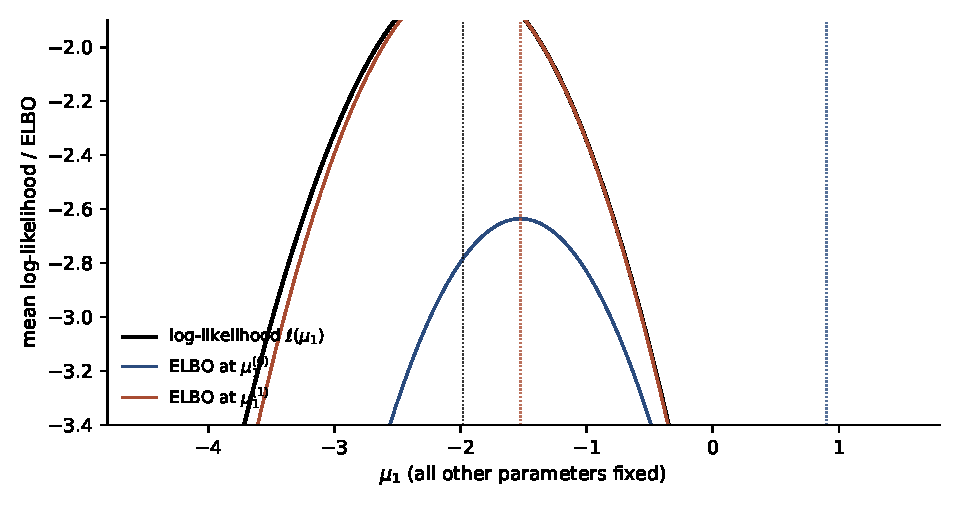
\includegraphics[width=0.86\linewidth]{figures/em_bound.pdf}
  \caption{\textbf{EM as bound tangency.} The mixture log-likelihood
  (black) over one coordinate ($\mu_1$; all else fixed), with the ELBO
  surrogates erected by two successive E-steps. Each surrogate touches
  $\ell$ at its anchor point and minorizes it everywhere else; maximizing
  the surrogate (the M-step) moves the anchor uphill. Note also what the
  figure quietly demonstrates: $\ell$ itself is multimodal --- the bound
  climbs to whichever peak its start point drains toward
  (Chapter~\ref{ch:symmetry}).}
  \label{fig:embound}
\end{figure}

\begin{origins}[EM before and after 1977]
Weighted-reassignment iterations for mixtures date at least to Newcomb
(1886); the modern formulation, name, and general monotonicity proof are
Dempster, Laird and Rubin, ``Maximum Likelihood from Incomplete Data via
the EM Algorithm'' (\emph{JRSS-B}, 1977) --- one of the most cited
statistics papers ever written, covering missing data, censoring, and
latent structure in one framework. The view used in this chapter --- EM as
coordinate ascent on a single objective $\mathcal{L}(q, \theta)$ over
\emph{both} arguments --- is due to Neal and Hinton, ``A View of the EM
Algorithm that Justifies Incremental, Sparse, and Other Variants'' (1998),
and it is the version that matters for us: once EM is coordinate ascent,
\emph{partial} steps in either coordinate remain valid, which is the door
through which stochastic gradients enter
(Section~\ref{sec:generalizedem}). The same objective under the name
``variational free energy'' is the foundation of variational inference at
large; Proposition~\ref{prop:elbo} is the small-print contract behind the
modern ELBO industry.
\end{origins}

\section{The gradient identity}\label{sec:fisher}

EM's closed-form M-step \eqref{eq:mstep} is a Gaussian-mixture privilege.
The thesis model's components are neural networks; no closed form will
exist. The bridge to gradient training is an identity worth proving twice.

\begin{proposition}[Fisher's identity]\label{prop:fisher}
For the mixture \eqref{eq:mixdensity},
\begin{equation}\label{eq:fisher}
  \frac{\partial \ell}{\partial \theta}
  \;=\; \sum_j \sum_k r_{jk}\,
  \frac{\partial}{\partial \theta}
  \log\bigl(\pi_k\, \gauss(y_j; \mu_k, \sigma_k^2)\bigr):
\end{equation}
the gradient of the incomplete-data log-likelihood equals the
responsibility-weighted gradient of the complete-data log-likelihood.
\end{proposition}

\begin{proof}
Differentiate one term of \eqref{eq:incomplete} directly. With
$p_{jk} = \pi_k \gauss(y_j; \mu_k, \sigma_k^2)$,
\[
  \frac{\partial}{\partial \theta} \log \sum_k p_{jk}
  = \frac{\sum_k \partial_\theta\, p_{jk}}{\sum_l p_{jl}}
  = \sum_k \frac{p_{jk}}{\sum_l p_{jl}}\,
    \frac{\partial_\theta\, p_{jk}}{p_{jk}}
  = \sum_k r_{jk}\, \partial_\theta \log p_{jk}. \qedhere
\]
\end{proof}

The one-line mechanism --- $\partial \log \sum_k a_k = \sum_k
(a_k/\sum a)\, \partial \log a_k$ --- says that \emph{differentiating
through a marginalization automatically performs posterior inference}: the
weights that appear are exactly the Bayes posterior. Nobody asks the
optimizer to compute responsibilities; they emerge from the chain rule.
This is the sense in which ``just take gradients of the NLL'' does not
bypass EM but contains it.

\section{Generalized EM, and EM as the trainer's semantics}
\label{sec:generalizedem}

Theorem~\ref{thm:em}'s proof used the M-step only through inequality (b):
any $\theta^{(t+1)}$ that \emph{improves} $\mathcal{L}(q^{(t)}, \cdot)$
--- not necessarily maximizes it --- preserves monotonicity. Algorithms of
this form are \emph{generalized EM} (GEM). One gradient step on the
expected complete-data log-likelihood improves it (for small enough step);
by Fisher's identity that gradient \emph{equals} the gradient of $\ell$
itself. Stacking the pieces:

\begin{center}
\emph{SGD on the mixture NLL is generalized EM in which the E-step is
implicit in the forward pass and the M-step is one gradient step.}
\end{center}

This sentence is the semantic contract of the package's training loop, and
it earns its box:

\begin{engineering}[the trainer is an EM loop wearing an optimizer]
The package never implements an E-step or an M-step. It implements a
forward pass that computes the joint scores $a_{jk} = \log \pi_k + \log
\gauss(y_j; \mu_k, \sigma_k^2)$, a fused loss $-\LSE_k(a_{jk})$, and a
call to \code{loss.backward()}. By Fisher's identity, autograd's gradient
is the responsibility-weighted complete-data gradient --- responsibilities
included, at the current parameters, for the current minibatch. AdamW's
update is a (preconditioned, momentum-carrying) partial M-step. What is
\emph{lost} relative to classical EM is the monotonicity guarantee ---
minibatch noise and adaptive step sizes void Theorem~\ref{thm:em}'s
inequality chain --- which is why the package's training diagnostics
(Chapter~10) monitor the NLL rather than assume it
falls. What is \emph{gained} is everything: neural components, minibatch
scaling, one optimizer for every module, and a single code path shared
with the HMM variant (Chapter~\ref{ch:hmm}). The trade was accepted with
its eyes open, and the vocabulary of this chapter --- ``the E-step is in
the forward pass'' --- is used verbatim in the design document.
\end{engineering}

\begin{codewalk}[nec\_moe/losses.py --- the fused objective]
The entire chapter compresses into eleven lines of the package:
\begin{lstlisting}
a = log_prior + log_lik            # (B, K): a_k = log pi_k + log N_k
lse = torch.logsumexp(a, dim=-1)   # (B,): log p(y | x), the evidence
per_sample = -lse                  # the NLL
log_filtered = a - lse.unsqueeze(-1)   # (B, K): log r, ATTACHED
return MixtureNLLOutput(
    nll=per_sample.mean(),
    per_sample_nll=per_sample,
    log_filtered=log_filtered,
    responsibilities=log_filtered.detach().exp(),  # diagnostics copy
)
\end{lstlisting}
Three deliberate choices. (i) \emph{Log domain end to end}: densities are
never exponentiated and re-logged; \code{logsumexp} subtracts the row
maximum internally, so the computation survives residuals that would
underflow \code{float64} densities (a fat-tailed return under a calm
component reaches $e^{-1500}$ without blinking). (ii) \emph{One fused
pass}: evidence and posterior come from the same tensor \code{a} ---
the E-step really is the forward pass. (iii) \emph{Two exits for $r$}:
\code{log\_filtered} stays attached to the graph because the HMM recursion
threads it forward in time (Chapter~\ref{ch:hmm}); \code{responsibilities}
is a detached probability-domain copy for dashboards, so no diagnostic can
ever become a second, accidental training signal.
\end{codewalk}

\section{What EM does not promise}\label{sec:empathology}

Two failure modes survive all of the above, and both have engineering
consequences that the package carries visibly.

\subsection{Local optima}

Theorem~\ref{thm:em} promises ascent, not summit. The mixture likelihood
is multimodal --- Figure~\ref{fig:embound} shows two peaks in a
\emph{one}-dimensional slice --- and both EM and SGD converge to the basin
of their initialization. For the thesis model the dominant mode of failure
is not a bad local peak but a \emph{symmetric saddle} that looks like
convergence; Chapter~\ref{ch:symmetry} is devoted to it. Flag planted
here: nothing in this chapter's theory prevents it.

\subsection{The likelihood is unbounded}

\begin{proposition}[Degenerate spikes]\label{prop:spike}
For $K \ge 2$, the Gaussian-mixture likelihood \eqref{eq:incomplete} is
unbounded above: $\sup_\theta \ell(\theta) = +\infty$.
\end{proposition}

\begin{proof}
Park component 1 on a data point: $\mu_1 = y_1$, and let
$\sigma_1 \to 0$ with all other parameters fixed and non-degenerate. The
$j = 1$ term contains $\pi_1 \gauss(y_1; y_1, \sigma_1^2) =
\pi_1 / (\sqrt{2\pi}\,\sigma_1) \to \infty$, so
$\log p(y_1) \to \infty$ at rate $\log(1/\sigma_1)$. Every other term is
bounded below by its (fixed, finite) other-component mass:
$\log p(y_j) \ge \log\bigl(\pi_2 \gauss(y_j; \mu_2, \sigma_2^2)\bigr) >
-\infty$. The sum diverges.
\end{proof}

The global ``optimum'' of the exact problem is therefore a pathology: one
component collapsing onto one observation with vanishing variance. MLE for
mixtures only makes sense as a search for a good \emph{interior} local
maximum, and every practical mixture fitter constrains scales away from
zero.

\begin{whatbreaks}[unconstrained $\sigma$]
A mixture fit on returns with free scales and an unlucky initialization
will manufacture a ``regime'' containing one crash day, $\sigma_k
\to 0$, NLL $\to -\infty$, and a model that is numerically dead (the next
forward pass overflows) while \emph{reporting its best loss ever} --- the
leakage ratchet's evil twin: an objective that rewards self-destruction.
The package's defenses are layered and mundane: $\sigma$ is parameterized
as $\log \sigma$ (positivity is structural, and the spike must travel
infinitely far in parameter space rather than to the boundary);
\code{sigma\_init} calibrates the starting scale to the target's standard
deviation; and \code{sigma\_freeze\_steps} holds $\log\sigma$ fixed during
early training --- the spike is most reachable when means are still
garbage, which is precisely when the freeze is on. The freeze keys off
\code{step\_count}, which is why checkpoint resume restoring
\code{step\_count} exactly (Chapter~10) is a correctness
requirement, not a convenience.
\end{whatbreaks}

\exercisehead

\begin{exercise}\label{ex:4-mstep}
Derive the M-step \eqref{eq:mstep} from \eqref{eq:elbo2}: (a) for
$\mu_k$ and $\sigma_k^2$ by direct differentiation; (b) for the weights
$\pi_k$ by maximizing $\sum_j \sum_k r_{jk} \log \pi_k$ subject to
$\sum_k \pi_k = 1$ with a Lagrange multiplier. (c) Where does the
constraint qualification fail if some component receives zero total
responsibility, and what does the package's load-balance \emph{monitoring}
(not the aux loss --- the dashboard) have to do with it?
\end{exercise}

\begin{exercise}\label{ex:4-fisher}
Prove Fisher's identity \eqref{eq:fisher} a second way: differentiate the
decomposition \eqref{eq:elbodecomp} with respect to $\theta$ at the point
$q = r(\theta_0)$, $\theta = \theta_0$, using the fact that the KL term is
minimized (hence has zero gradient) there. Conclude that the ELBO and
$\ell$ have identical gradients wherever the bound touches --- the reason
one gradient step after an E-step is a GEM step.
\end{exercise}

\begin{exercise}\label{ex:4-handem}
By hand, run two full EM iterations for a $K = 2$ mixture with fixed
$\sigma_1 = \sigma_2 = 1$, $\pi = (\tfrac12, \tfrac12)$, on the four
observations $y = (-2, -1, 1, 2)$ from the start $\mu = (-0.5, 0.5)$.
Report the responsibilities and means at each step. Then argue (no
computation) where the iteration converges, and what would happen instead
from the start $\mu = (0, 0)$ --- you have met this phenomenon before, and
you will meet it again in Chapter~\ref{ch:symmetry}.
\end{exercise}

\begin{exercise}\label{ex:4-spike}
Quantify Proposition~\ref{prop:spike}'s spike: with $\mu_1 = y_1$ and
$\sigma_1 = \epsilon$, show $\ell$ grows as $\log(1/\epsilon) + O(1)$, and
compute how small $\epsilon$ must be for the spike to beat an interior
optimum by $\Delta$ nats. Then explain why the same spike is
\emph{harder} (but not impossible) to reach for the conditional model of
Chapter~\ref{ch:moe}, where $\mu_k(\cdot)$ is a shared function across
observations rather than a free scalar.
\end{exercise}

\begin{exercise}\label{ex:4-numpy}
(Hands-on.) Implement classical EM \eqref{eq:resp}--\eqref{eq:mstep} in
$\sim$25 lines of numpy. Generate $n = 2{,}000$ points from a two-regime
scale mixture (Chapter~\ref{ch:regimes}'s world, means zero,
$\sigma = (0.5, 2.5)$), and (a) verify monotonicity numerically at every
iteration; (b) compare the fixed point against the package's SGD route:
build a \code{ClassicalGaussianEmission} $\times$ \code{uniform}-prior
model on the same data and train with \code{Trainer.fit}; both should
recover $\sigma \approx (0.5, 2.5)$ up to permutation. (c) Time both.
Reflect: what did SGD buy, and what did it cost, on a problem where EM has
closed forms?
\end{exercise}

\begin{exercise}\label{ex:4-kl}
The E-step was derived as ``set $q$ to the posterior.'' Show it is also
the solution of $\min_q \mathrm{KL}(q \,\|\, r)$ trivially, and --- less
trivially --- that among all product distributions $q(z_{1:n}) = \prod_j
q_j(z_j)$, coordinate ascent on \eqref{eq:elbodecomp} recovers exactly the
per-observation posteriors, i.e.\ mean-field structure costs nothing here.
Why does this stop being true for the HMM of Chapter~\ref{ch:hmm}, where
the latent states are chained?
\end{exercise}
